\section{วิธีการไฟไนต์ดิฟเฟอเรนจ์เบื้องต้น}
\hspace{1cm}

\hspace{1cm} วิธีการไฟไนต์ดิฟเฟอเรนจ์ (finite difference method) ถูกคิดค้นโดย เป็นวิธีการเชิงตัวเลขที่พัฒนาขึ้นเพื่อแก้ไขปัญหาค่าขอบ ซึ่งทั่วไปแล้วขั้นตอนของวิธีการไฟไนต์ดิฟเฟอเรนซ์สำหรับการแก้ปัญหาค่าขอบประกอบดวยสามขั้นตอนสำคัญดังนี้

\begin{enumerate}
    \item ดิสครีตไทซ์ (discretize) โดเมนของผลเฉลย (solution domain) ออกเป็นช่องตาราง (mesh) ของจุดกริด (grid point) ที่ต้องการหาผลเฉลยเชิงตัวเลข
    \item ประมาณอนุพันธ์ที่ปรากฏในปัญหาค่าขอบด้วยการประมาณแบบไฟไนต์ดิฟเฟอเรนซ์ (finite difference approximation) ในขั้นตอนนี้ การประมาณดังกล่าวจะนำไปสู่ระบบสมการเชิงเส้น หรือระบบสมการไม่เป็นเชิงเส้นขนาดใหญ่ที่สมนัยกับปัญหาค่าขอบตั้งต้น
    \item แก้ระบบสมการเชิงเส้นหรือระบบสมการไม่เป็นเชิงเส้นขนาดใหญ่ที่เกิดขึ้นในขั้นตอนที่ 2 เพื่อกำหนดผลเฉลยเชิงตัวเลข
\end{enumerate}

\hspace{1cm} กำหนดให้ $u(x)$ แทนฟังก์ชันค่าจริงและเป็นฟังก์ชันราบเรียบ (smooth function) นั่นคือ $u$ สามารถหาอนุพันธ์ได้หลายครั้ง โดยแต่ละครั้ง อนุพันธ์ที่หาได้เป็นฟังก์ชันที่ถูกนิยามอย่างดี (well-defined) และมรขอบเขตเหนือช่วงที่มีจุดที่สนใจ $\bar{x}$

\hspace{1cm} ในการประมาณ $u'(\bar{x})$ โดยใช้ค่าของ $u$ ที่เกิดจากจุดที่อยู่ในบริเวณใกล้เคียงกับ $\bar{x}$ สามารถใช้สูตรการประมาณแบบไฟไนต์ดิฟเฟอเรนซ์ที่ถูกกำหนดได้ดังต่อไปนี้
\begin{enumerate}
    \item สูตรฟอร์เวิร์ดดิฟเฟอเรนซ์ (forward-difference formular) 
    \begin{align*}
        D_{+}u(\bar{x}) = \frac{u(\bar{x}+h) - u(\bar{x})}{h}    
    \end{align*}
    \item สูตรแบ็คเวิร์ดดิฟเฟอเรนซ์ (backward-difference formular) 
    \begin{align*}
        D_{-}u(\bar{x}) = \frac{u(\bar{x}) - u(\bar{x}-h)}{h}    
    \end{align*}
    \item สูตรเซ็นทรัลดิฟเฟอเรนซ์ (forward-difference formular) 
    \begin{align*}
        D_{0}u(\bar{x}) = \frac{u(\bar{x}+h) - u(\bar{x}-h)}{2h}    
    \end{align*}
\end{enumerate}
โดยที่ $h$ เป็นจำนวนจริงที่มีค่าน้อยๆ ซึ่ง $h>0$ 

\hspace{1cm} สำหรับโครงงานวิจัยนี้ จะใช้วิธีการหาอนุพันธ์โดยประมาณไฟไนต์ดริฟเฟอเรนจ์แบบฟอร์เวิร์ดดิฟเฟอร์เรน จึงได้ว่าการหาอนุพันธ์ของค่าความเข้มที่พิกัดทางกายภาพเป็น $(i,j)$ สามารถหาได้ดังนี้
\begin{align*}
	\frac{d}{dx} u_{i,j} = \frac{u_{i,j+1} - u_{i,j}}{h}
\end{align*}

เมื่อระบบกริดที่ใช้บนภาพมีความห่างเพียงหนึ่งหน่วย จึงได้ว่า $h=1$ ทั้งนี้ระยะห่าง $h$ อาจเปลี่ยนไปตามชั้นของพีระมิดรูปภาพ

\begin{figure}[H]
    \centering
    \begin{subfigure}{0.95\linewidth}
        \centering
        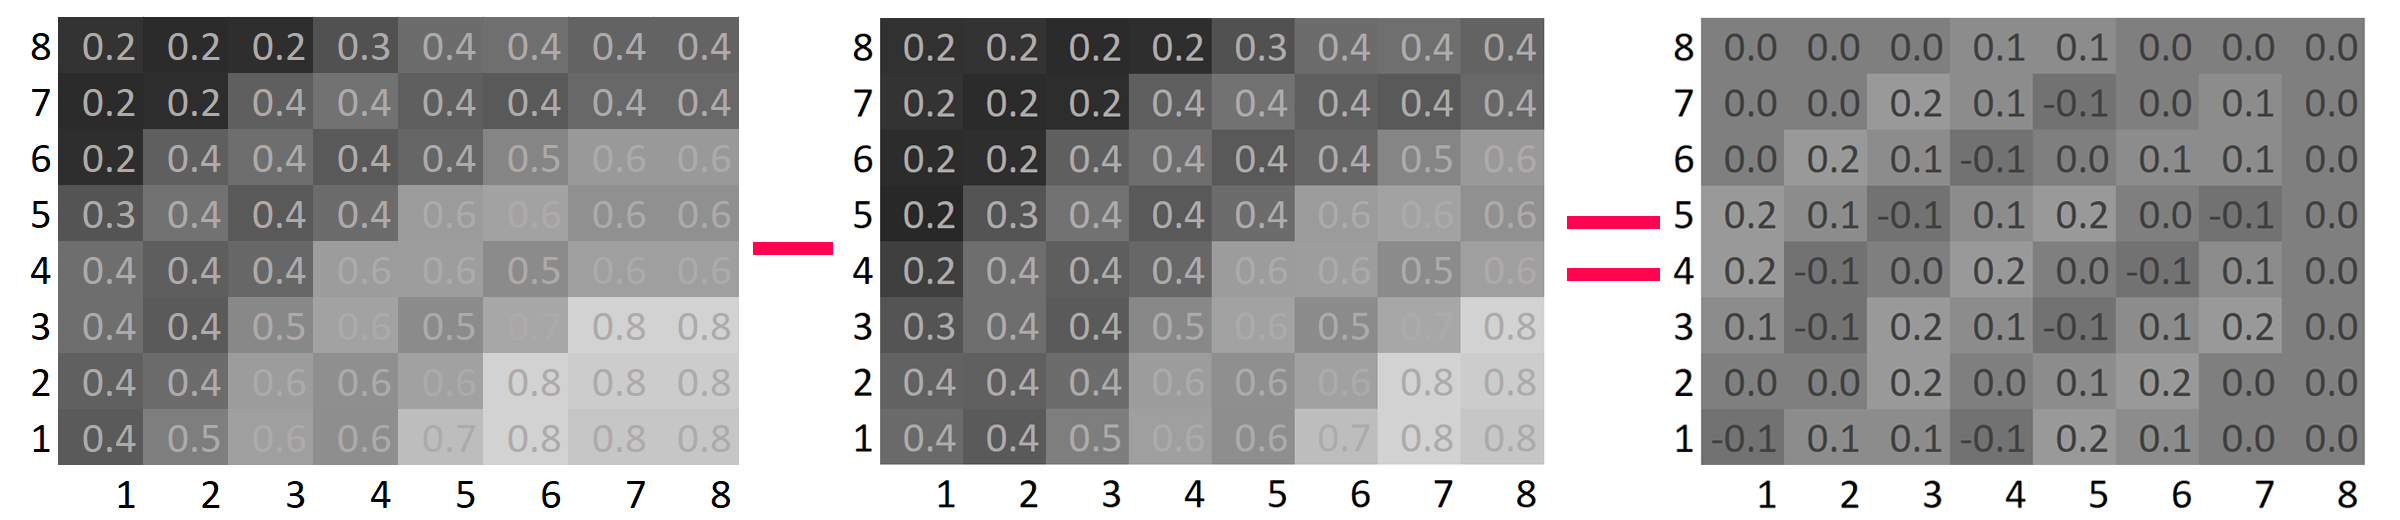
\includegraphics[width=0.9\linewidth]{image/finite_difference/x_derivertive.png}
    \end{subfigure}
    \caption{ตัวอย่างการหาอนุพันธ์บนภาพเฉดเทา}
    \label{figure:x-derivertive}
\end{figure}

\hspace{1cm} จากภาพ \ref{figure:grayscale-explain} เมื่อต้องการหาอนุพันธ์เทียบแกน x จะทำตามภาพที่ \ref{figure:x-derivertive}โดยทำการสร้างภาพซึ่งทำการตัดขอบทางซ้ายออกหนึ่งคอลัมม์และเพิ่มขอบทางขวาหนึ่งคอลัมม์โดยใช้เงื่อนไขค่าขอบแบบนิวแมน จากนั้นภาพที่สร้างขึ้นไปลบกับภาพเดิมจะได้อนุพันธ์ของภาพนั้นดังที่ปรากฏทางขวา ทั้งนี้หาก $ h \neq 1 $ สามารถทำการหารภาพผลลัพธ์ด้วยค่า $h$ ได้เพื่อให้ได้ค่าที่ต้องการ

\noindent\hspace{1cm}สำหรับการหาเกรเดียนซ์ (Gradient) จะใช้การหาอนุพันธ์โดยวิธีฟอร์เวิร์ดดิฟเฟอร์เรนจ์ดังที่กล่าวไปในข้างต้น ในแนวแกน x และแนวแกน y คำตอบที่ได้จะเป็นเวคเตอร์ของอนุพันธ์แนวแกน x และอนุพันธ์แนวแกน y  ได้เวคเตอร์ดังนี้ 
\begin{align*}
	\nabla \vec{v_{u_i}} = (\frac{\partial }{\partial x} u_{i,j},\frac{\partial}{\partial y} u_{i,j})^{\top}	
\end{align*}

\noindent\hspace{1cm}สำหรับไดเวอร์เจน (Divergence) จะเป็นการหาผลรวมของอนุพันธ์ในแต่ละแกนของเวคเตอร์ด้วยวิธีฟอร์เวิร์ดดิฟเฟอร์เรนจ์ นั่นคือ 
\begin{align*} 
	\nabla \cdot (\vec{v_{i,j}}) = \frac{\partial}{\partial x}\vec{v_{i,j}}_x + \frac{\partial}{\partial y}\vec{v_{i,j}}_y
\end{align*}

\noindent\hspace{1cm}สำหรับลาปาเซียน (Lapacian) นั่นคือการทำหาไดเวอร์เจนบนเวคเตอร์ที่หาแกรเดียนแล้ว แต่ทั้งนี้สามารถหาลาปาเชียนได้จาก

\begin{align*}
	\triangle u_{i,j} = u_{i-1,j} + u_{i+1,j} + u_{i,j-1} + u_{i,j+1} - 4 u_{i,j} 
\end{align*}



